\documentclass[usenames,dvipsnames, aspectratio=169, 9pt]{beamer}
\beamertemplatenavigationsymbolsempty
\setbeamertemplate{footline}[frame number]
\setbeamertemplate{section in toc}[sections numbered]
\usecolortheme[named=Plum]{structure}
\usefonttheme{serif}
\usepackage{amsmath, amsthm, amssymb, pgffor, multirow, booktabs, tabularx, multirow, graphicx, pgffor, arydshln}
\usepackage{kotex}
\usepackage{epstopdf}
\usepackage{grffile}


\author{Boyeon Kim}
\institute{Department of Mathematics, School of Mathematics and Computing \\ Mathematics \\ Yonsei University}
%\date{January 6, 2023}
\title{Reinforcement Learning Seminar}

\def\bs{\boldsymbol}
\usepackage{grffile}
\begin{document}

  \maketitle
\begin{frame}{SLIAR Optimal control}
    \begin{itemize}
        \item Goal1 : Reproduce the SLIAR optimal control by uning PMP
        \item Method : PMP (Adjoint)
    \end{itemize}
\end{frame}


\begin{frame}\frametitle{SLIAR Model}
    \begin{itemize}
        \item SLIAR Model Equations and structure.
    \end{itemize}
    $\begin{cases}
        S' &= -\beta (1-\sigma) S\Lambda - \nu S\\
        L' &= \beta (1-\sigma) S\Lambda - \kappa L\\
        I' &= p\kappa L - \alpha I - \tau I \\
        A' &= (1-p)\kappa L - \eta A \\
   \end{cases}$ \qquad with $\Lambda = \epsilon L + (1 - q) I + \delta A$
    \centering
    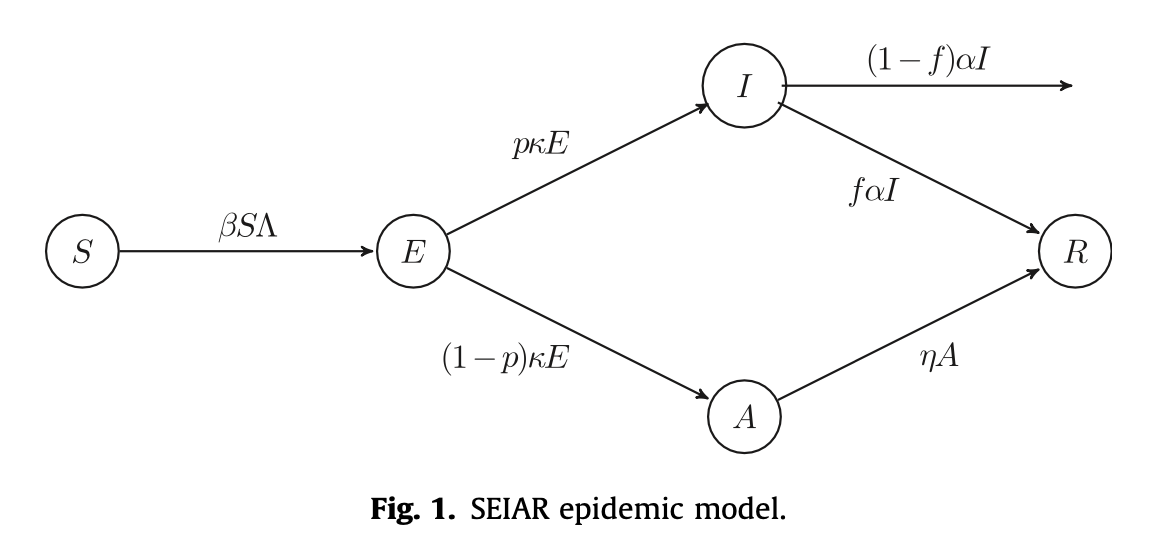
\includegraphics[width=10cm]{figure/sliar_diag.png}
\end{frame}


\begin{frame}\frametitle{SLIAR model parameters}
    \begin{table}
\centering
\begin{tabular}{rllrl}
Start & 0      & &$\beta$         & 7.26e-07  \\
End   & 300    & &$\sigma$        & 0         \\
S0    & 1e06    & &$\kappa$        & 0.526     \\
L0    & 0      & &$\alpha$        & 0.224     \\
I0    & 1      & &$\tau_{max}$ & 0.05      \\
A0    & 0      & &$\nu_{max}$  & 0.01 \\
$R_0$  & 1.9847 & &$\epsilon$      & 0.224     \\
$P$ & 1      & &$q$                            & 0.5       \\
$Q$ & 1e06    & &$p$        & 0.667         \\
$R$ & 1e06    & &$\delta$        & 1   \\
$W$ & 0   &     &                             &          
\end{tabular}
\end{table}
\end{frame}


\begin{frame}\frametitle{SLIAR w/o constrol}
    \centering
    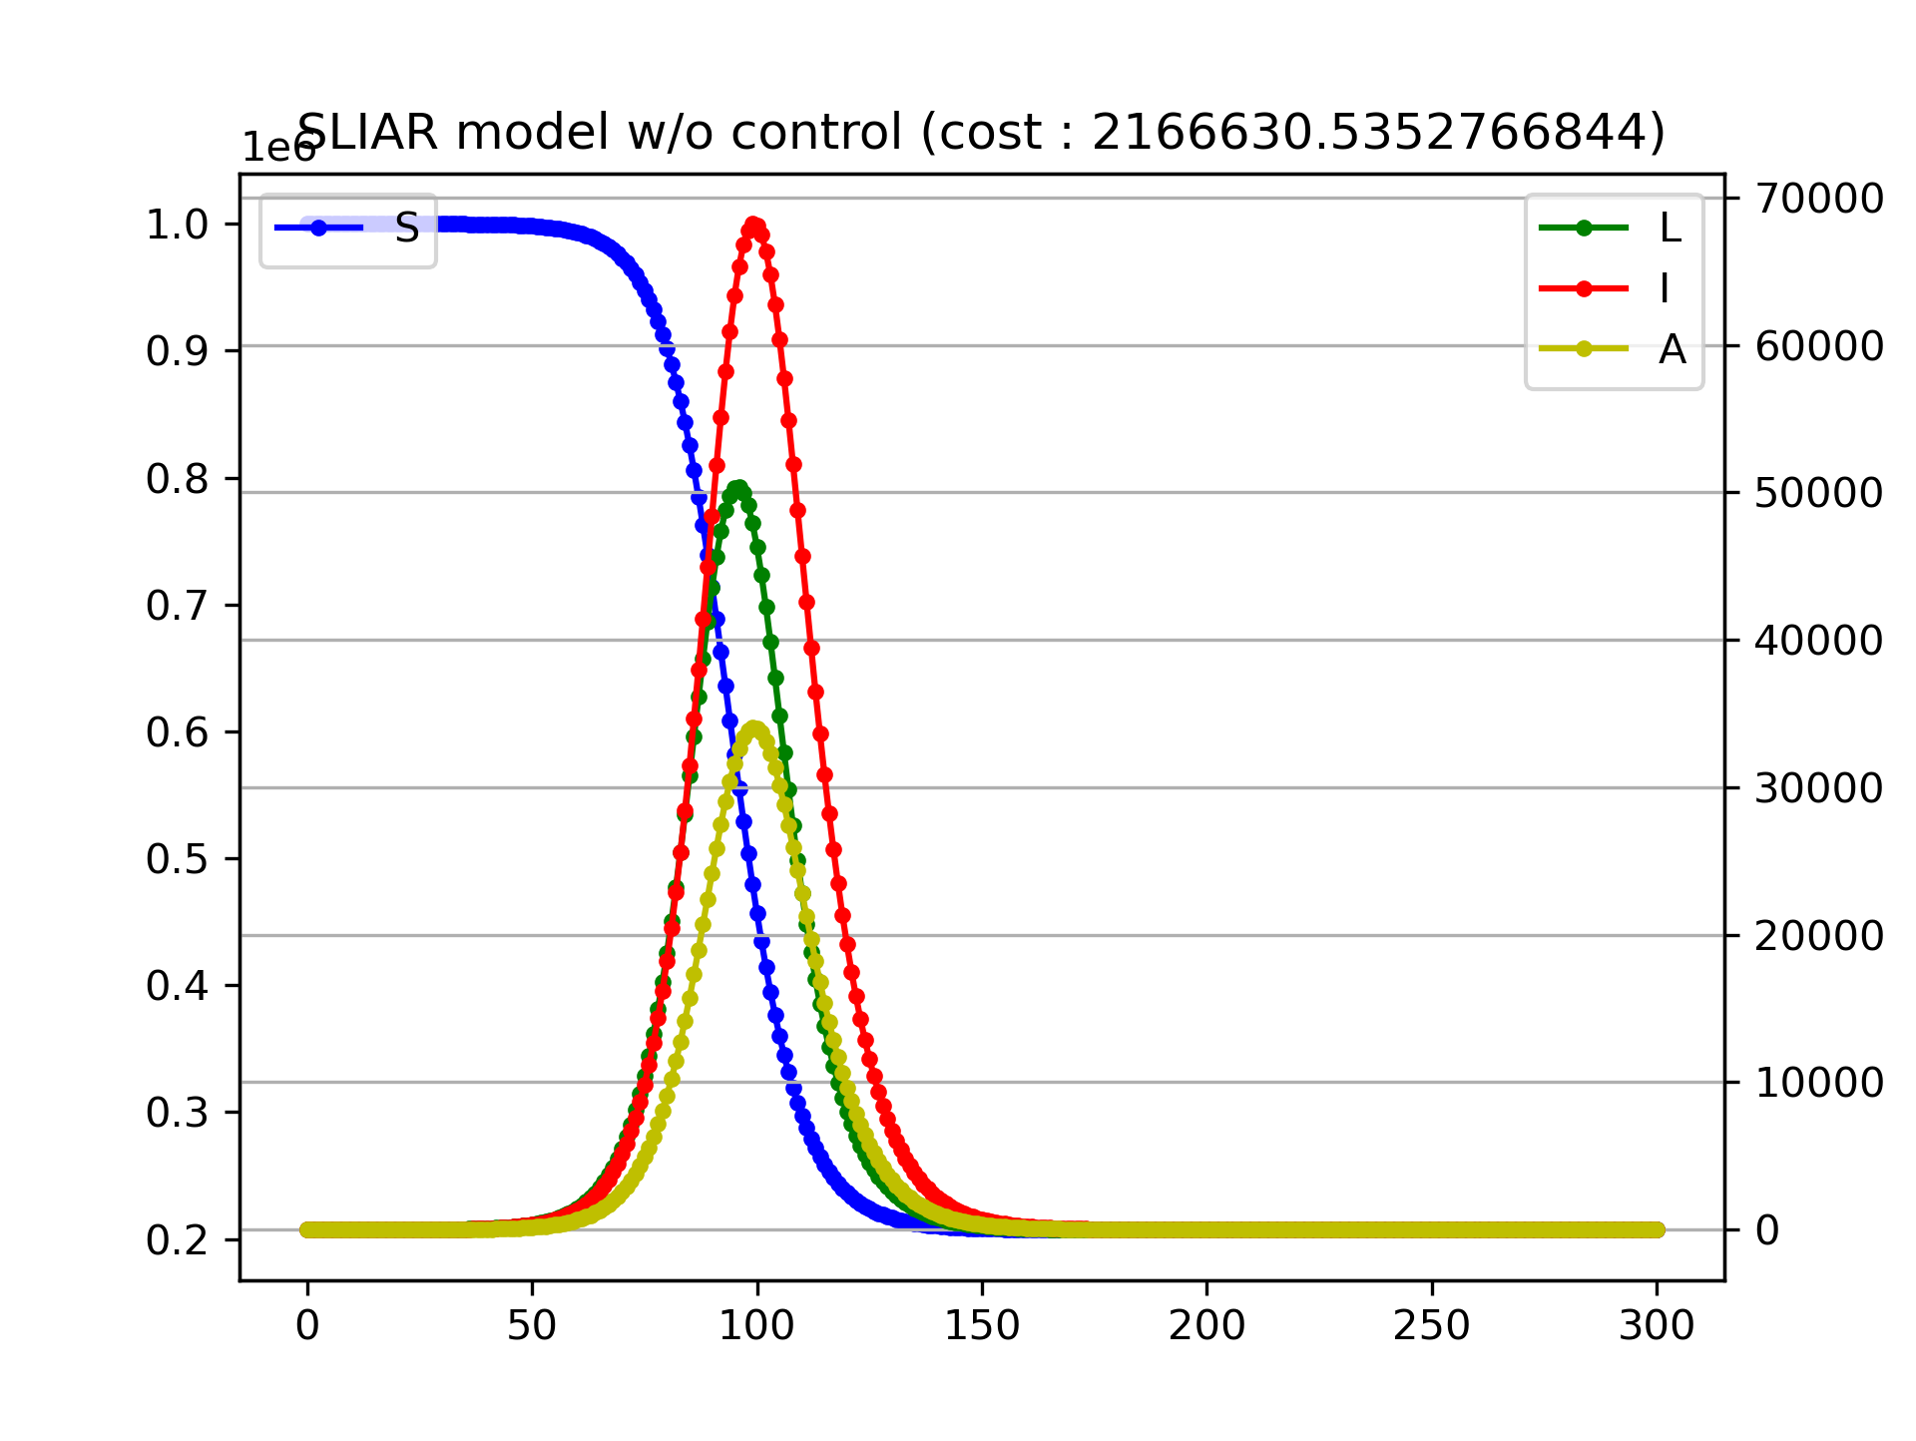
\includegraphics[width=10cm]{figure/sliar_wo_control.png}
\end{frame}


\begin{frame}\frametitle{SLIAR optimal control}
\begin{align*}
\min_{u\in\mathcal{U}_{ad}} \int_0^T PI(t) + Q\nu^2(t) + R\tau^2(t) + W\sigma^2(t) dt
\end{align*}

    subject to 
    \begin{align*}
    \begin{cases}
        S' &= -\beta (1-\sigma) S\Lambda - \nu S\\
        L' &= \beta (1-\sigma) S\Lambda - \kappa L\\
        I' &= p\kappa L - \alpha I - \tau I \\
        A' &= (1-p)\kappa L - \eta A \\
   \end{cases} \qquad with \quad \Lambda = \epsilon L + (1 - q) I + \delta A
   \end{align*}
\end{frame}

\foreach \e in {0.1, 0.001, 1e-04, 1e-06} {
        \begin{frame}\frametitle{SLIAR optimal control}
        \begin{itemize}
        \item $ \min_{u\in\mathcal{U}_{ad}} \int_0^T PI(t) + Q\nu^2(t) + R\tau^2(t) + W\sigma^2(t) dt$
        \item Method : PMP(Adjoint)
        \item P = 1, Q = 1E6, R = 1E6, $\nu_{max} = 0.01$, learning rate : \e
        \end{itemize}
        
            \centering
            \includegraphics[width=6cm]{figure/adjoint/\e/costs.png}
        
        \end{frame}
}

\begin{frame}{SLIAR Optimal control}
    \begin{itemize}
        \item Goal2 : 2-constraint optimal control 
        \item Method : DQN
    \end{itemize}
\end{frame}

\foreach \e in {2000, 5000, 7000, 10000} {
        \begin{frame}\frametitle{SLIAR optimal control}
        \begin{itemize}
        \item $ \min_{u\in\mathcal{U}_{ad}} \int_0^T PI(t) + Q\nu^2(t) + R\tau^2(t) + W\sigma^2(t) dt$
        \item Method : DQN
        \item P = 1, Q = 1E6, R = 1E6, $\nu_{max} = 0.01$, $\tau_{max} = 0.05$,iteration : \e
        \end{itemize}
        
            \centering
            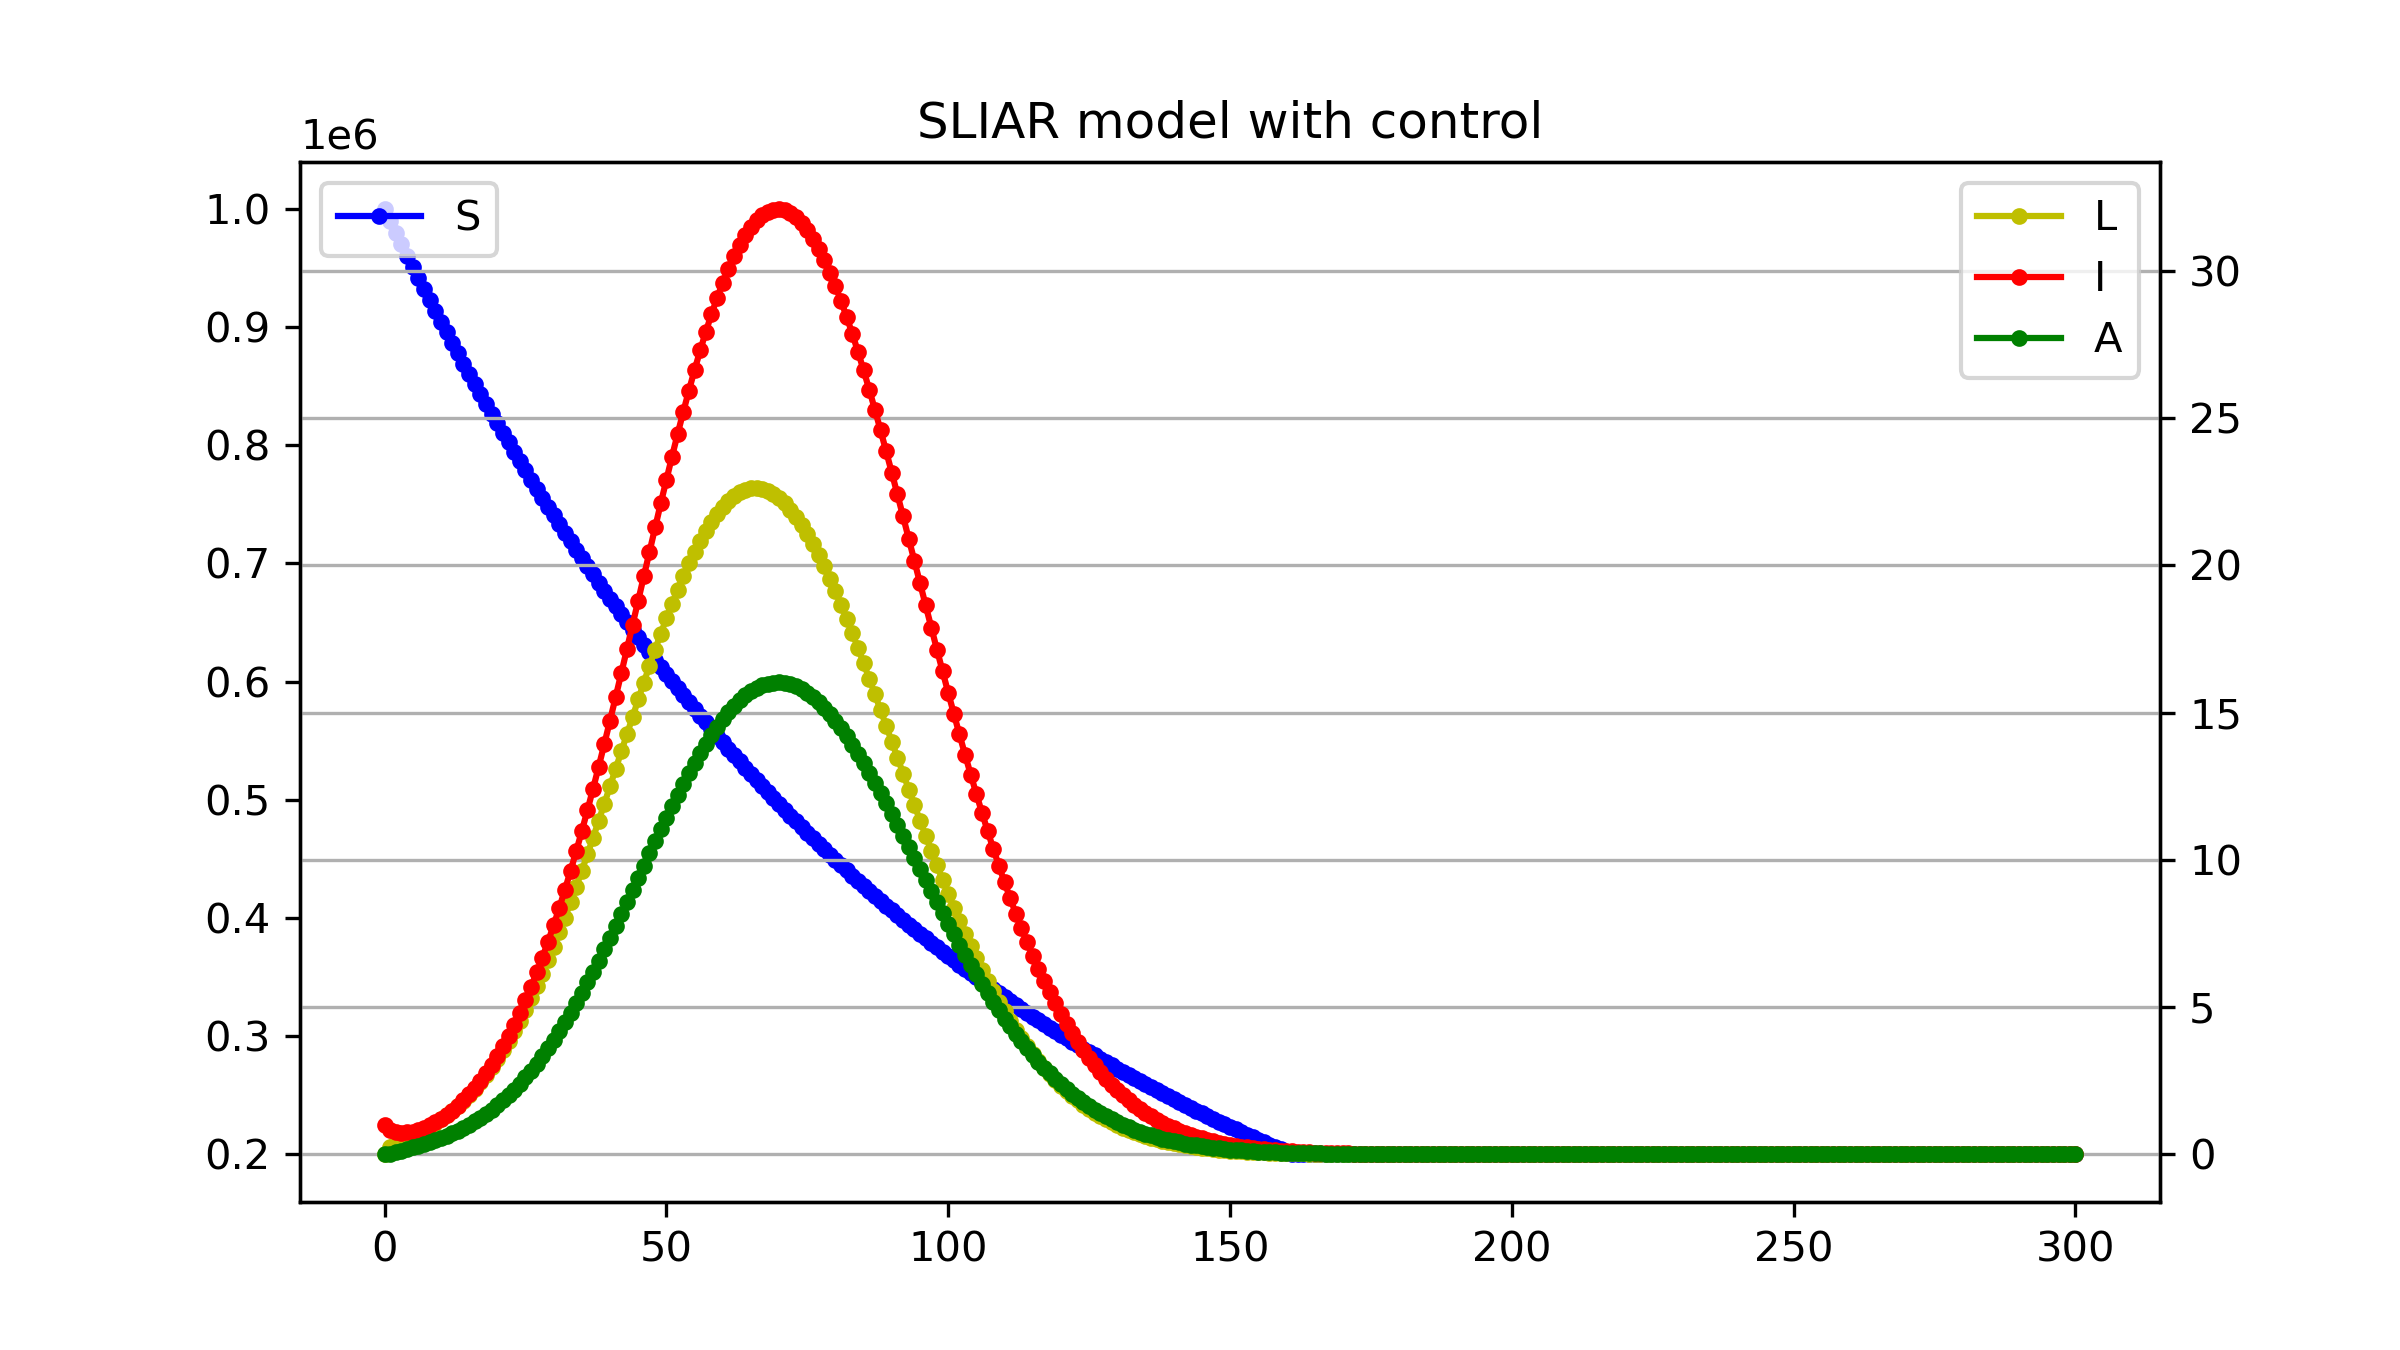
\includegraphics[width=6cm]{figure/multi/\e/SLIAR_w_control.png}
            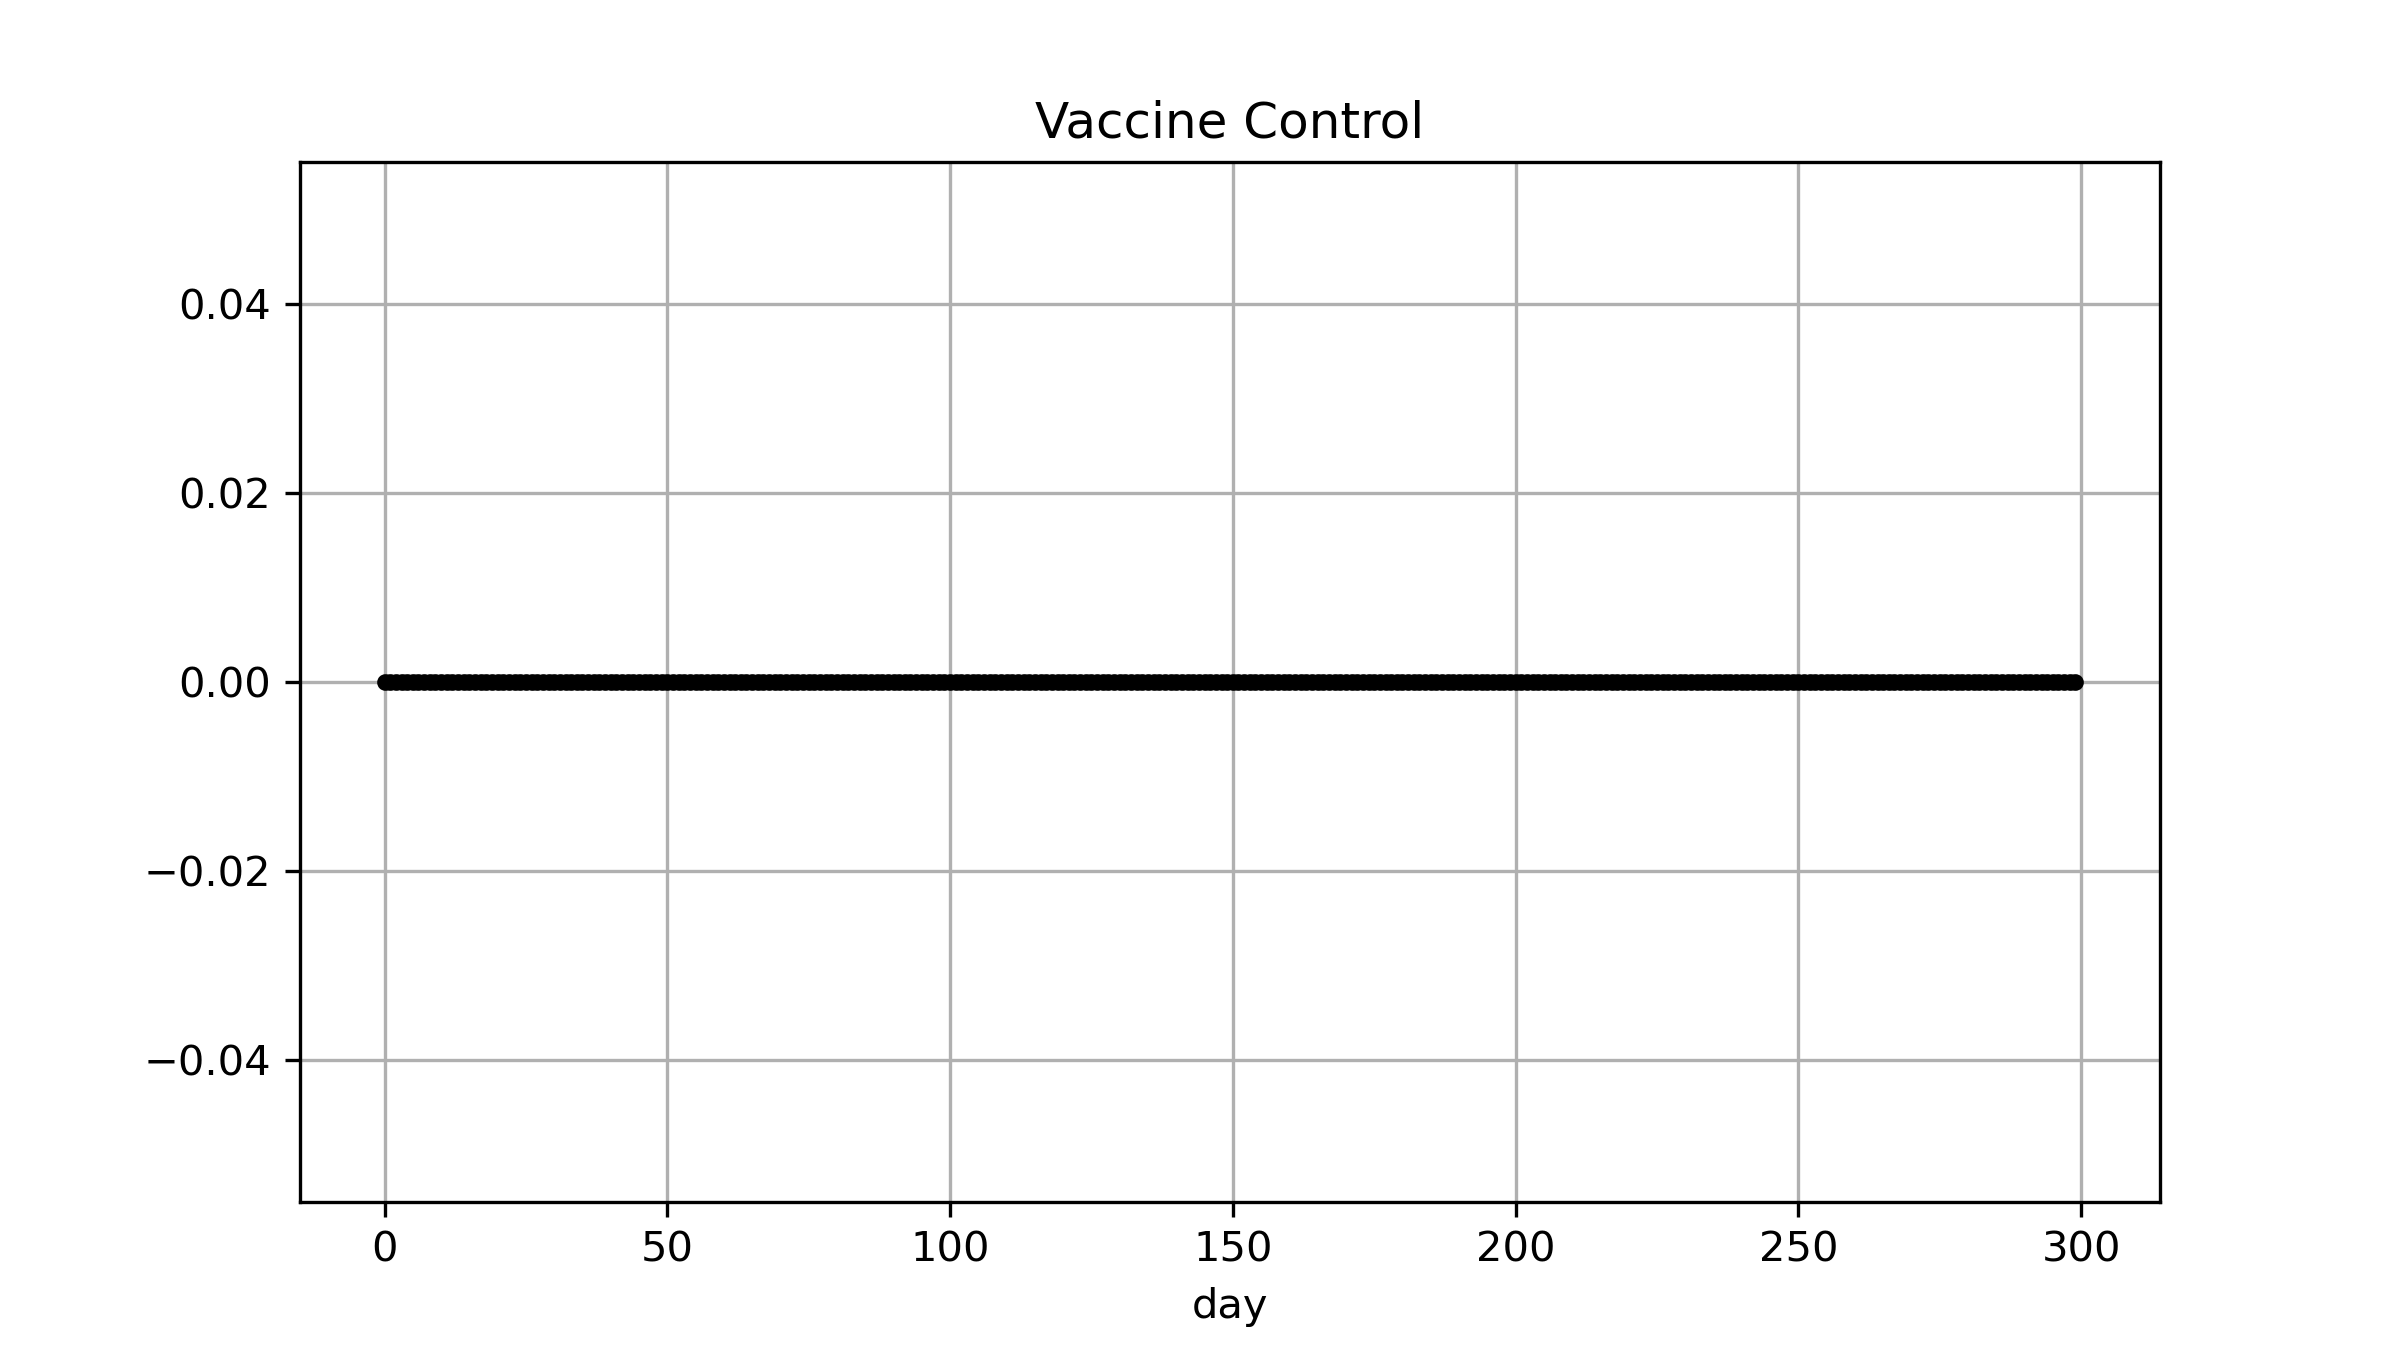
\includegraphics[width=6cm]{figure/multi/\e/SLIAR_control_u.png}
        
        \end{frame}
}

\begin{frame}\frametitle{1-constraint result of DQN}
\begin{itemize}
\item $ \min_{u\in\mathcal{U}_{ad}} \int_0^T PI(t) + Q\nu^2(t) + R\tau^2(t) + W\sigma^2(t) dt$
\item Method : DQN
\item P = 1, Q = 1e6, R = 1e6 $\nu_{max} = 0.01$, iteration : 10,000
\end{itemize}
    \centering
    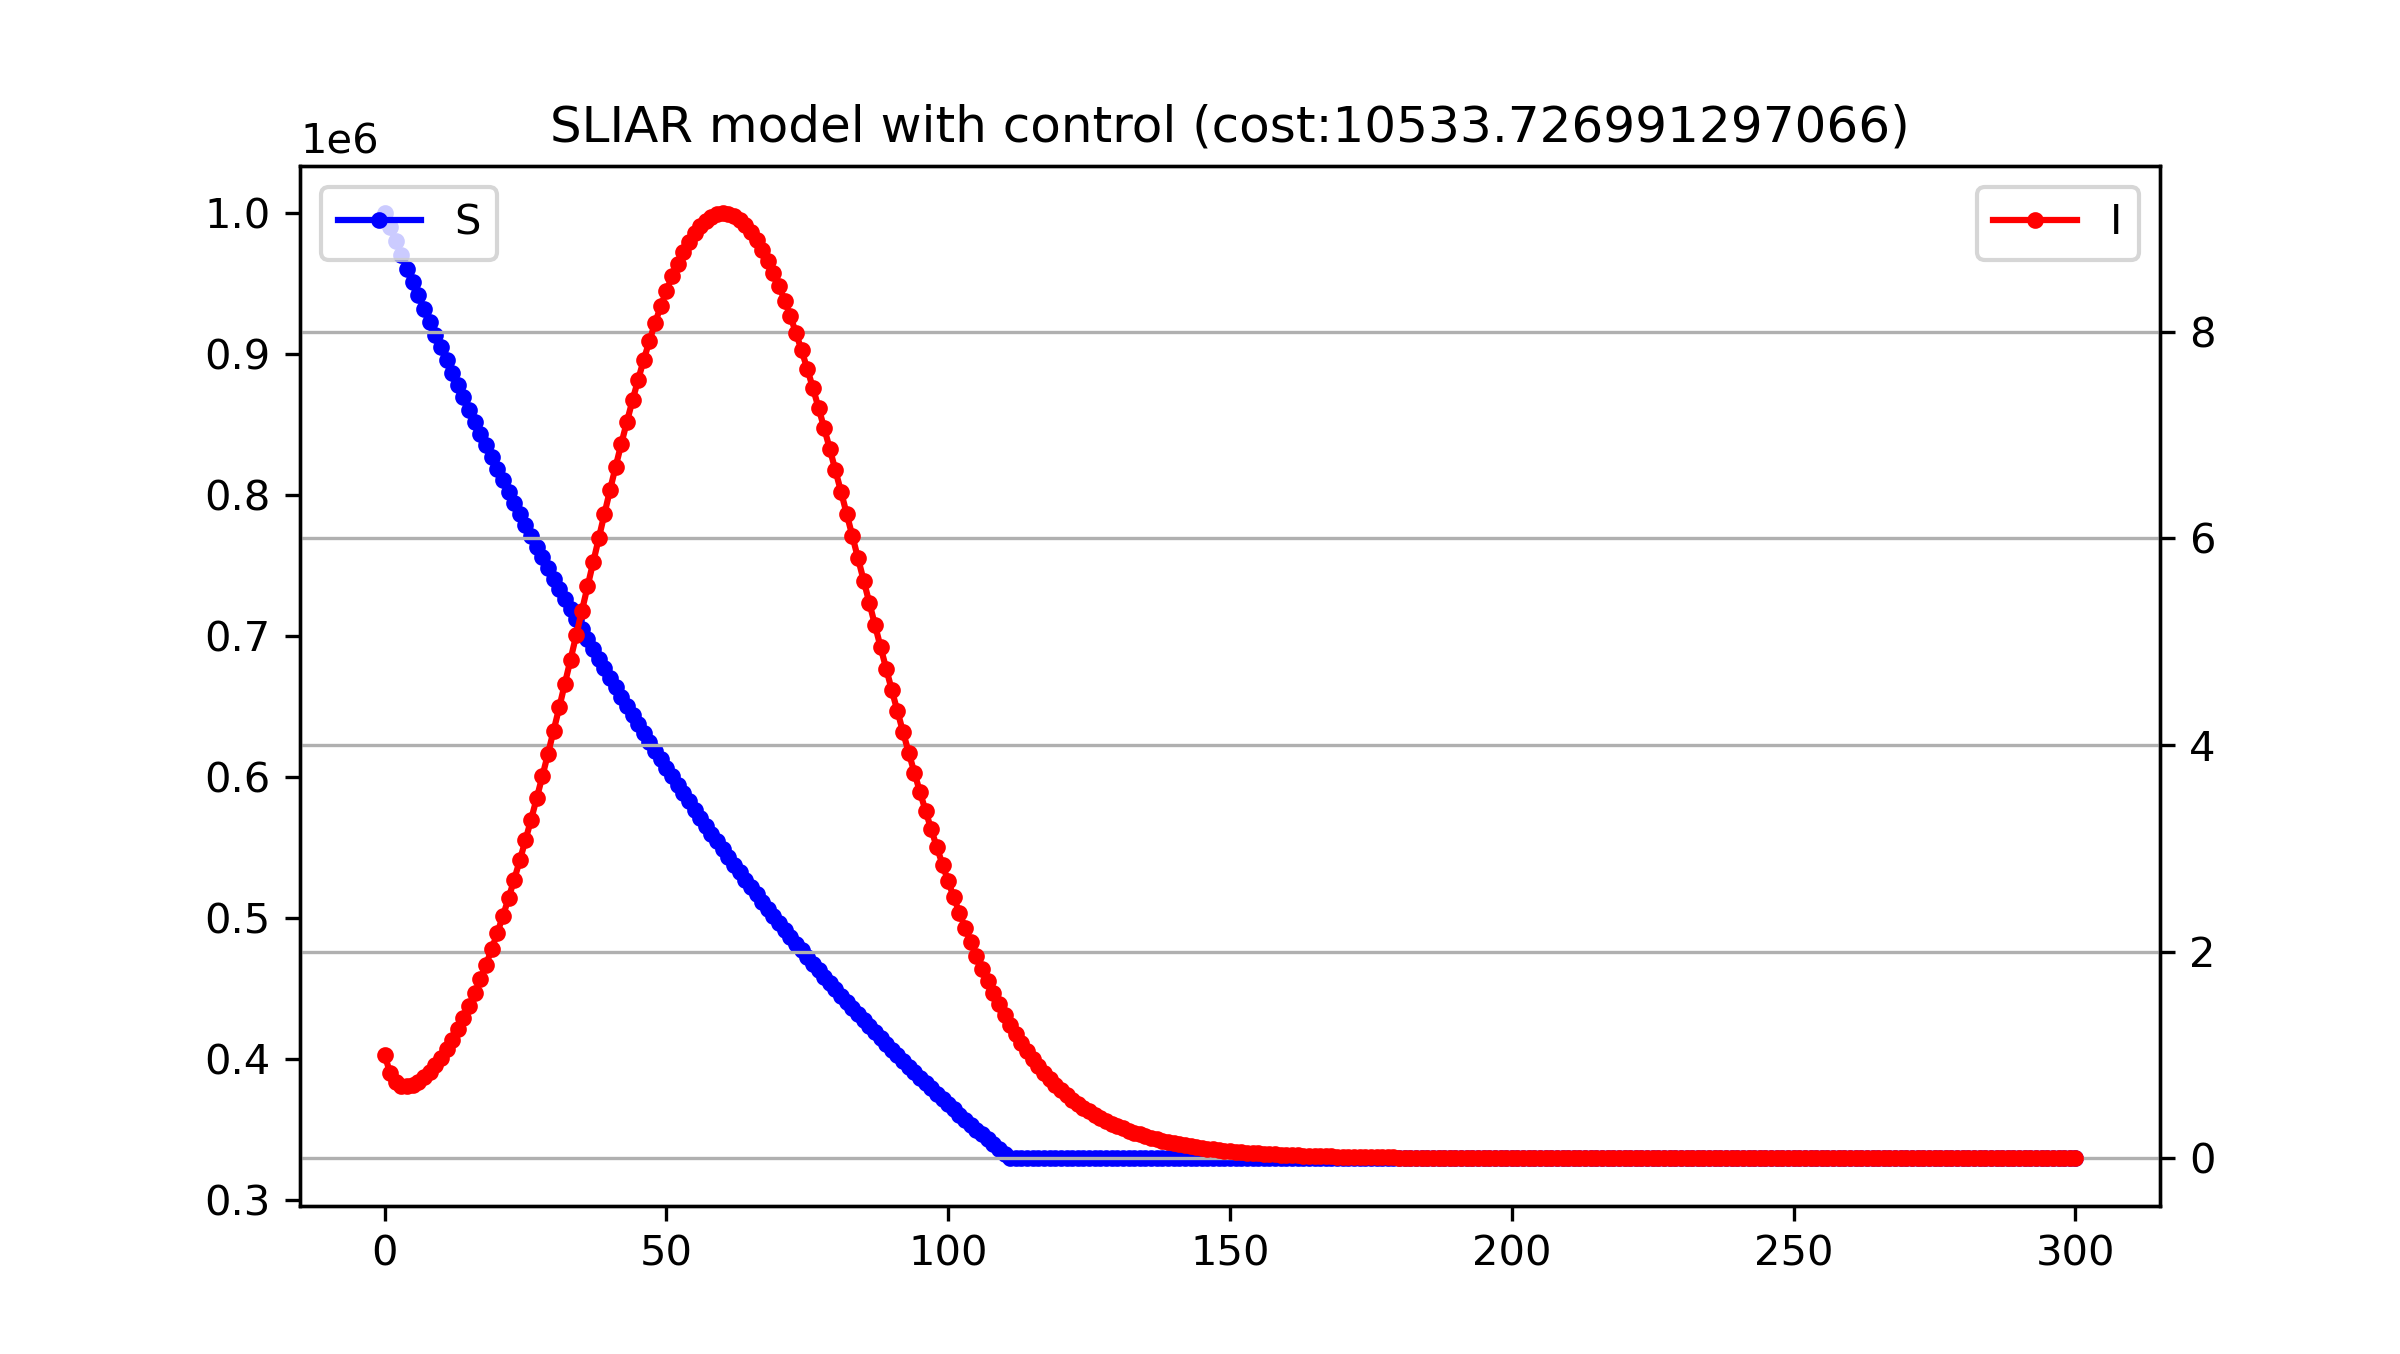
\includegraphics[width=6.5cm]{figure/sliar_dqn_numax.png}
    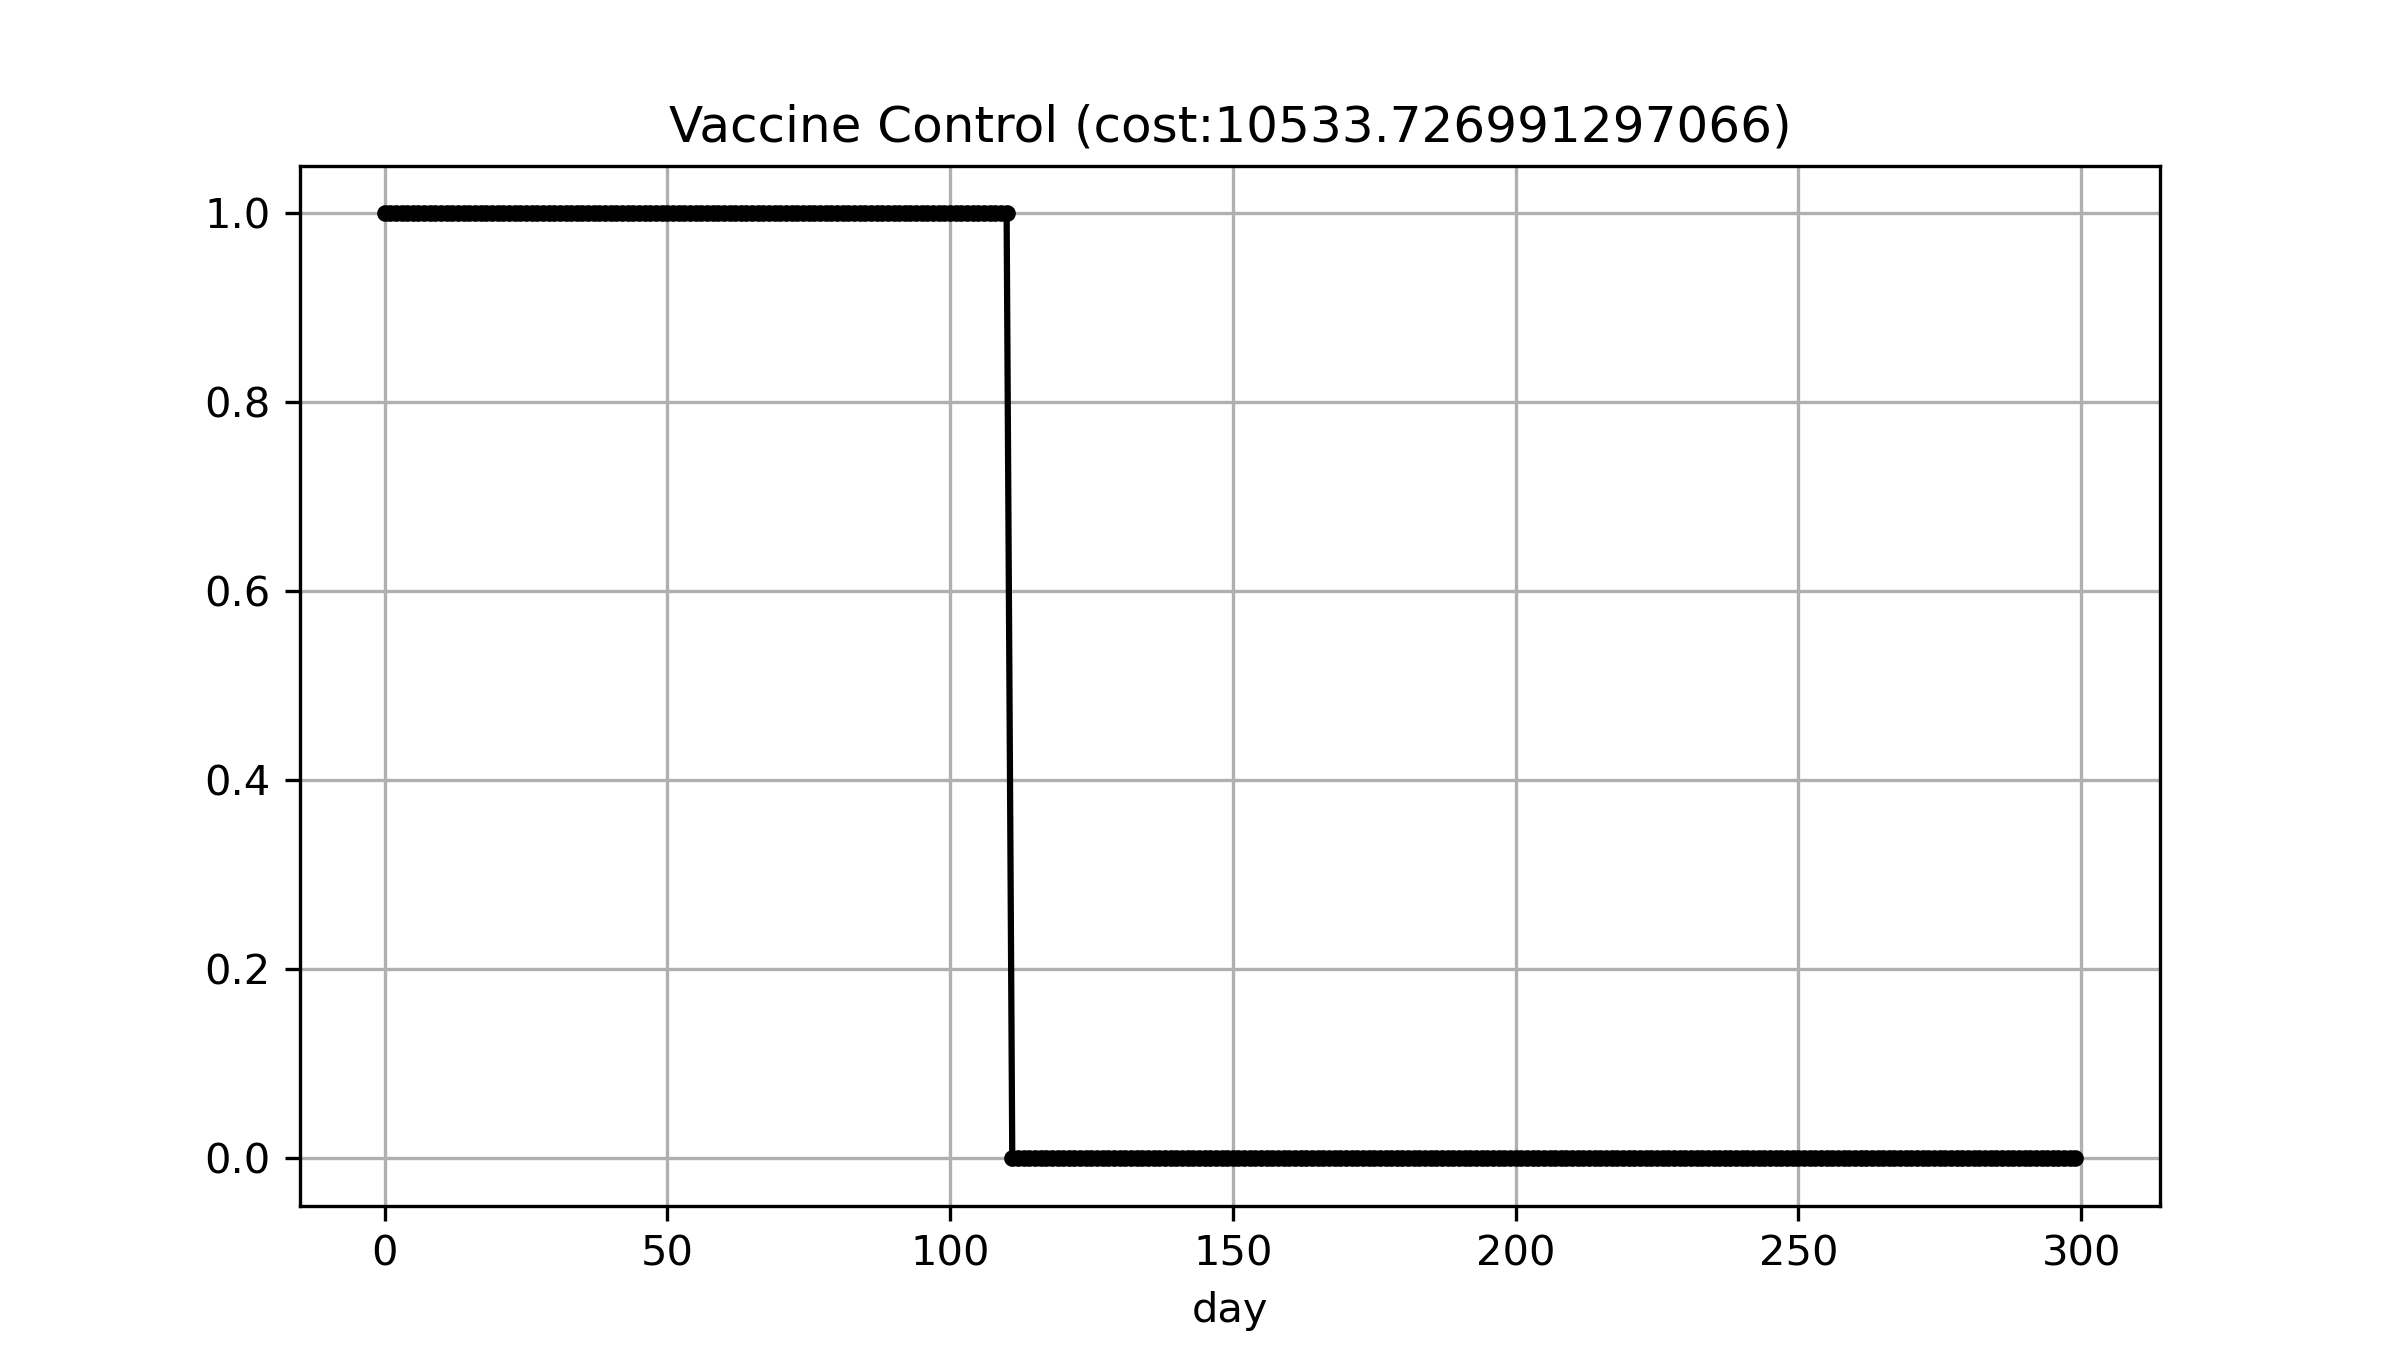
\includegraphics[width=6.5cm]{figure/sliar_dqn_numax_control.png}
\end{frame}

\begin{frame}\frametitle{1-constraint result of DQN}
\begin{itemize}
\item $ \min_{u\in\mathcal{U}_{ad}} \int_0^T PI(t) + Q\nu^2(t) + R\tau^2(t) + W\sigma^2(t) dt$
\item Method : DQN
\item P = 1, Q = 1e6, R = 1e6$\tau_{max} = 0.05$, iteration : 10,000
\end{itemize}
    \centering
    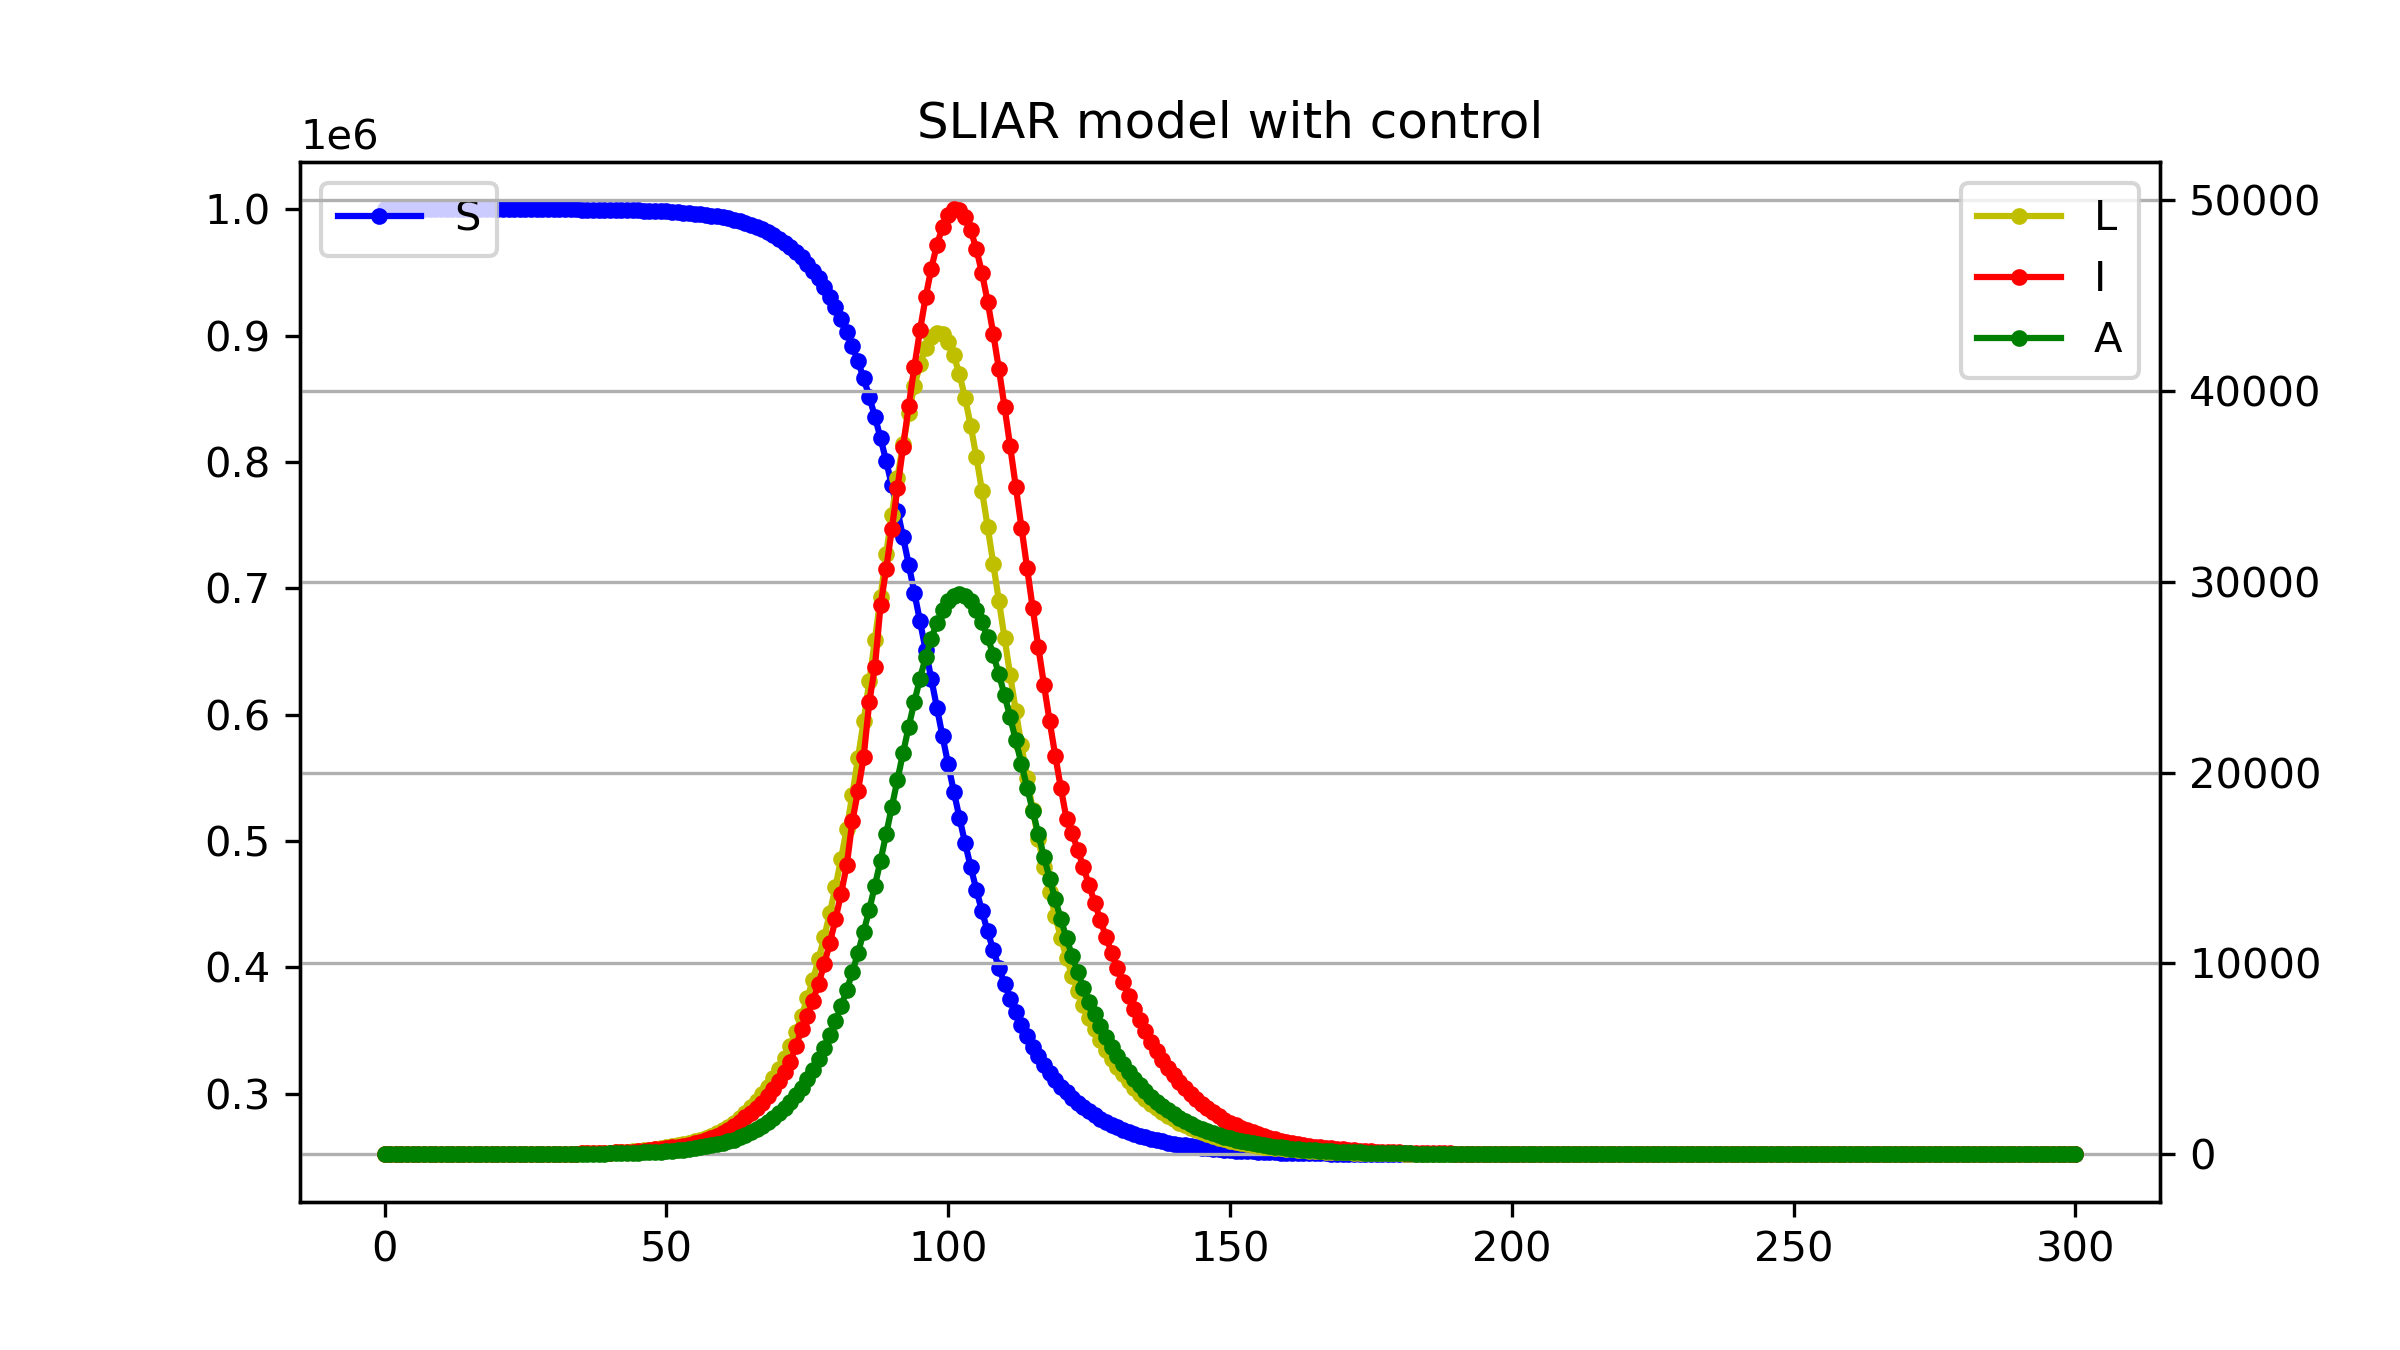
\includegraphics[width=6.5cm]{figure/sliar_dqn_tau.png}
    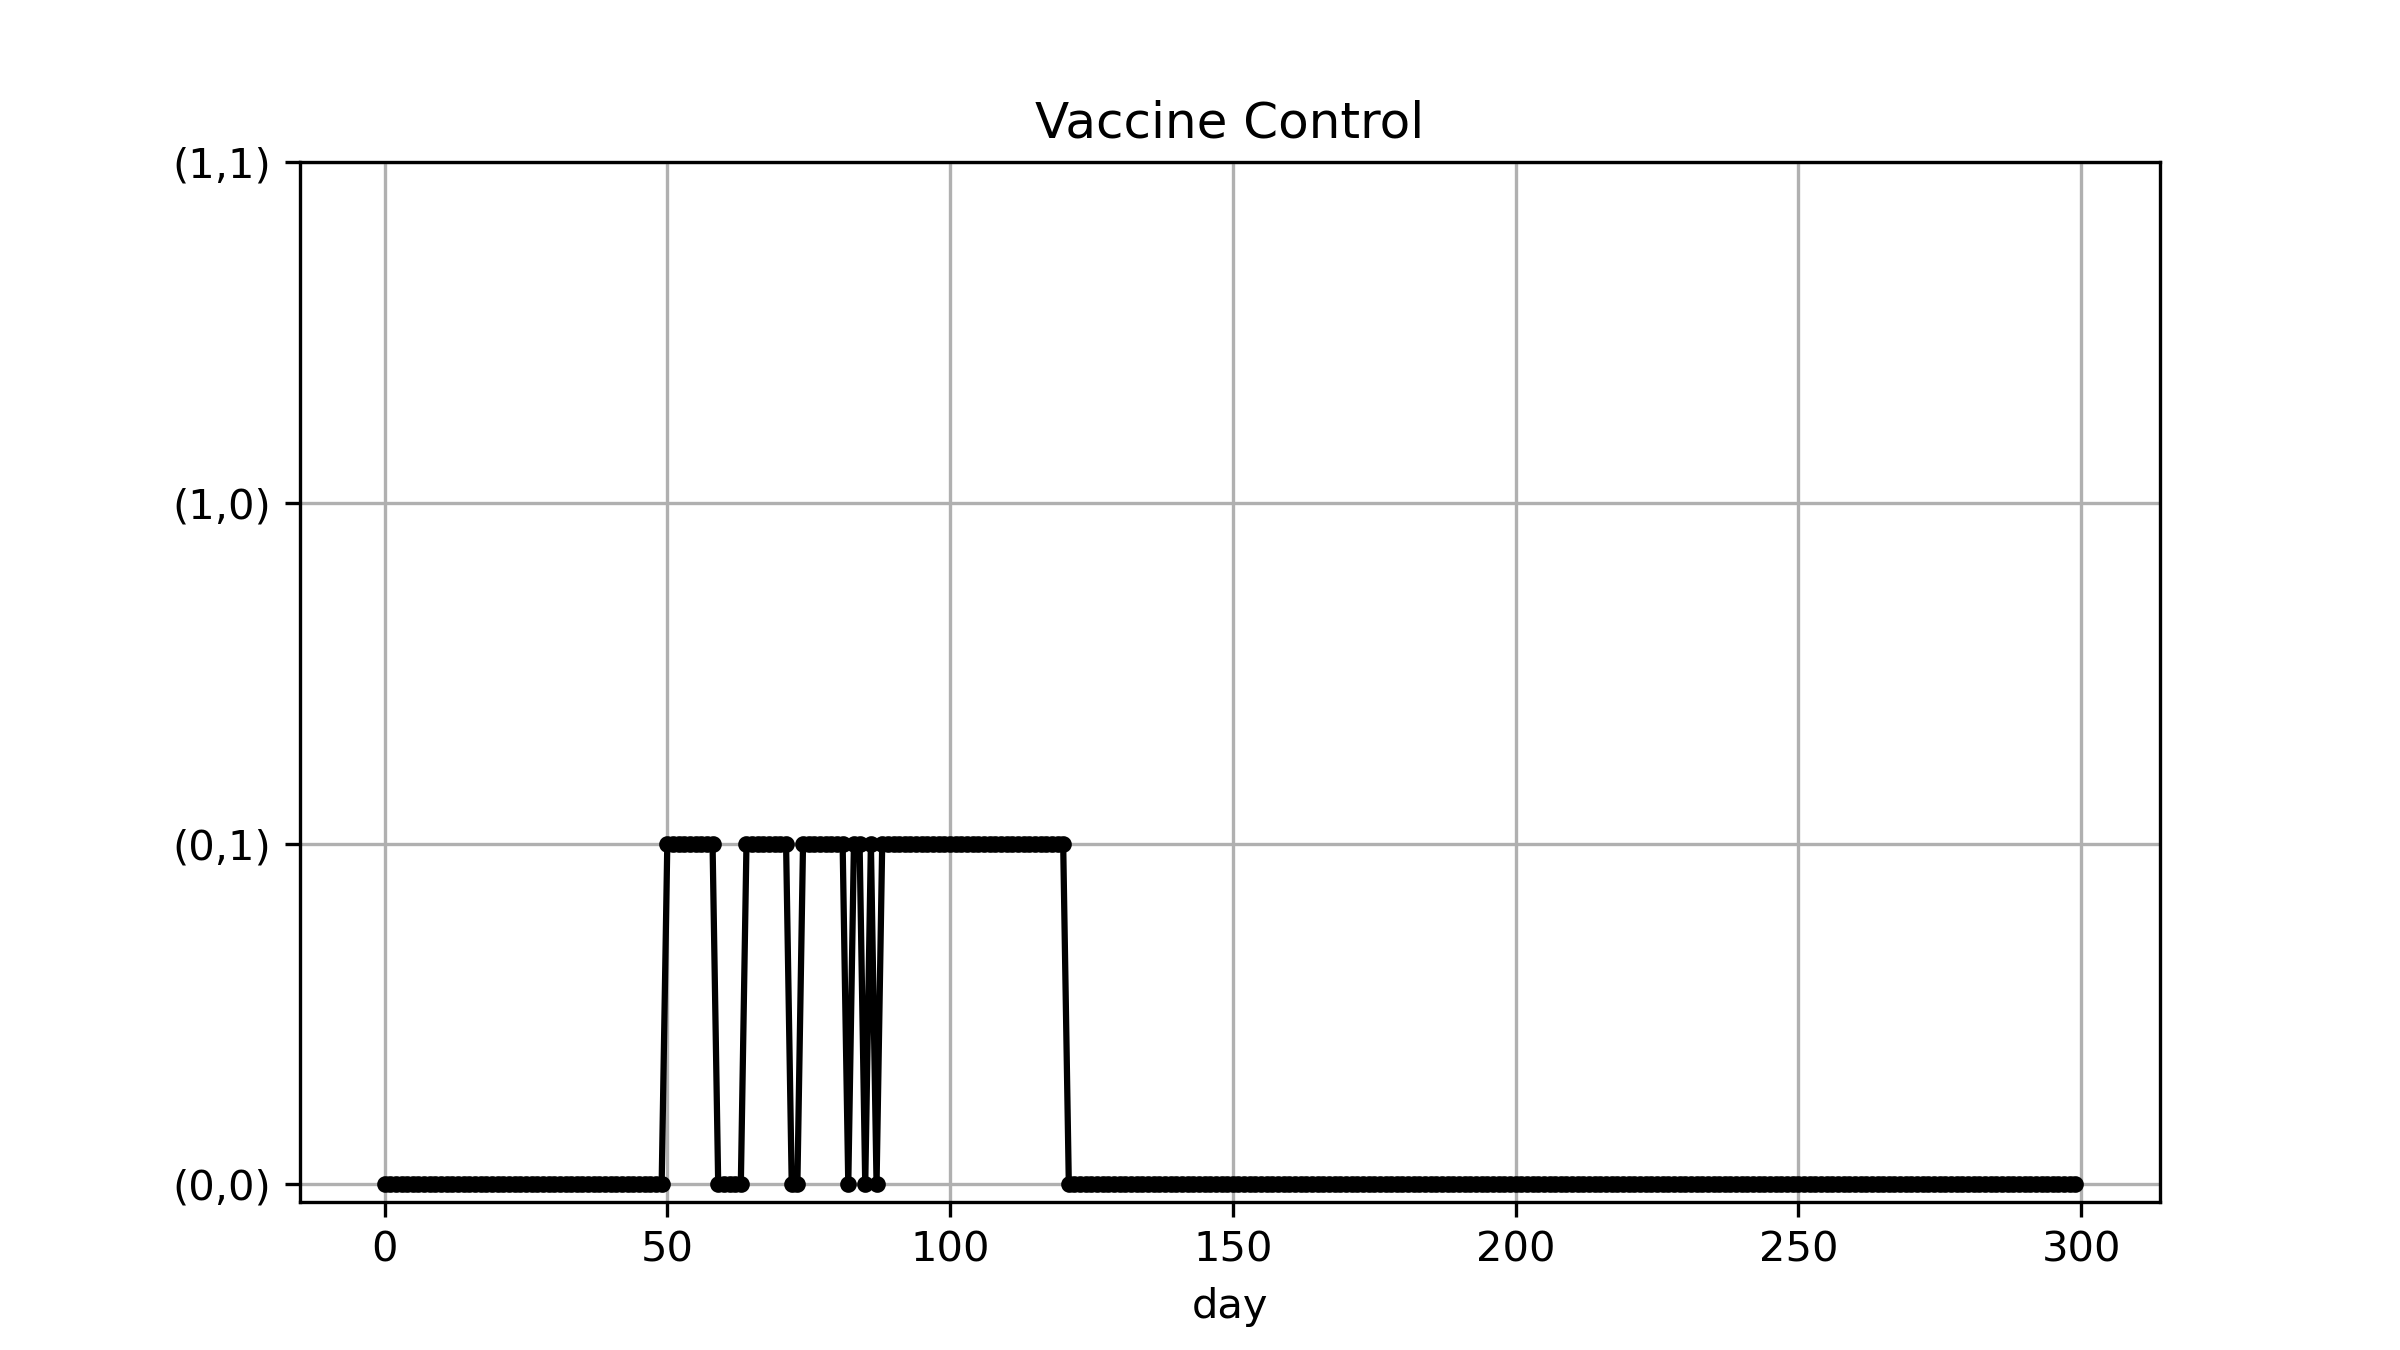
\includegraphics[width=6.5cm]{figure/sliar_dqn_tau_control.png}
\end{frame}

\end{document}